\documentclass[aspectratio=169,10pt]{beamer}
\usetheme{Madrid}
\usecolortheme{seahorse}
\usefonttheme{professionalfonts}

\usepackage[utf8]{inputenc}
\usepackage{amsmath,amssymb,amsthm}
\usepackage{graphicx}
\usepackage{listings}
\usepackage{xcolor}
\usepackage{booktabs}
\usepackage{array}

\graphicspath{{figures/}}

\setbeamertemplate{footline}[frame number]
\setbeamertemplate{navigation symbols}{}

\lstset{
  basicstyle=\ttfamily\scriptsize,
  numbers=left,
  numberstyle=\tiny\color{gray},
  frame=single,
  backgroundcolor=\color{gray!7},
  commentstyle=\color{green!50!black}\itshape,
  keywordstyle=\color{blue},
  stringstyle=\color{orange!80!black},
  breaklines=true,
  showstringspaces=false,
  language=Python,
  tabsize=2
}

\newcommand{\Kc}{\mathcal{K}}
\newcommand{\Nc}{\mathcal{N}}

\title[E-Values -- Ch.9]{Hypothesis Testing with E-Values}
\subtitle{Chapter 9: FDR Control using Compound E-Values}
\author{Based on Ramdas \& Wang}
\date{}

\begin{document}

\begin{frame}
\titlepage
\end{frame}

\begin{frame}{Outline}
\tableofcontents
\end{frame}

% ============================================================
\section{Preliminaries}
% ============================================================

\begin{frame}[allowframebreaks]{Why we need something beyond single-hypothesis testing}

\textbf{Intuition.} So far in this book we tested \emph{one} hypothesis at a time with a single e-value. In practice, scientists rarely test just one thing: a genomics lab tests thousands of genes at once, a trading firm evaluates hundreds of strategies at once, a quality-control team checks dozens of production lines at once. If you test $K$ hypotheses at level $\alpha$ each, purely by chance you expect around $K\alpha$ false rejections even when \emph{every} hypothesis is null. With $K=1000$ and $\alpha=0.05$, that is about 50 false alarms -- an unacceptable number if you then trust every rejection at face value.

\vspace{2mm}
\textbf{The question this chapter answers:} if we have one e-value (or more generally a ``compound'' e-value) per hypothesis, how do we combine them into a single multiple-testing procedure that controls a sensible aggregate error notion, no matter how the hypotheses/tests are statistically entangled with one another?

\vspace{2mm}
\textbf{Roadmap.}
\begin{itemize}
\item 9.1: the basic object (compound e-values) and the main procedure (e-BH).
\item 9.2: every valid procedure secretly \emph{is} e-BH (a universality result).
\item 9.3: how to build the best possible compound e-values in a stylized model.
\item 9.4--9.6: three ways to squeeze more discoveries out of e-BH for free (adaptivity, randomization, closure).
\end{itemize}

\framebreak

\textbf{Setting up the scene.} We observe data $X$ (the entire dataset) drawn from some unknown $\mathbb{P}^\dagger$. We want to test $K$ null hypotheses simultaneously:
\[
H_k : \mathbb{P}^\dagger \in \mathcal{P}_k, \qquad k \in \Kc := \{1,\dots,K\}.
\]
Each $\mathcal{P}_k$ is a set of candidate distributions consistent with ``hypothesis $k$ is true.'' The (unknown) index set of \emph{true} null hypotheses is
\[
\Nc(\mathbb{P}) = \{k \in \Kc : \mathbb{P} \in \mathcal{P}_k\}, \qquad K_0 = |\Nc(\mathbb{P})|.
\]
Nothing here assumes independence across $k$: the $K$ tests can be built from the same dataset, from overlapping data, or from entirely dependent processes (e.g. correlated stock returns, or genes on the same biological pathway).

\end{frame}

% ============================================================
\begin{frame}[allowframebreaks]{Notation you'll need}

\textbf{Intuition first: the spam-filter analogy.} Suppose a spam filter flags 100 incoming emails as spam. Some of those 100 really are spam (correct rejections of ``this is not spam''); some are perfectly innocent emails that got flagged by mistake (false discoveries). The \emph{false discovery rate} (FDR) asks: \emph{on average, what fraction of the flagged emails are actually not spam?} If the filter always flags 100 emails and, on average, 5 of them are legitimate, the FDR is $5\%$. This is exactly the right way to think about the FDR in multiple hypothesis testing: ``discoveries'' = rejected hypotheses, and we want only a small fraction of them to be false alarms.

\begin{block}{False discovery proportion (FDP) and false discovery rate (FDR)}
Let $\mathcal{D} \subseteq \Kc$ be the (random) set of hypotheses that a procedure rejects (the ``discoveries''). Define
\[
F_{\mathcal{D}} = |\Nc(\mathbb{P}) \cap \mathcal{D}| \quad (\text{number of \emph{false} discoveries}), \qquad R_{\mathcal{D}} = |\mathcal{D}| \quad (\text{total discoveries}).
\]
\[
\text{FDP} = \frac{F_{\mathcal{D}}}{R_{\mathcal{D}} \vee 1}, \qquad \text{FDR} = \mathbb{E}^{\mathbb{P}}[\text{FDP}].
\]
Here $F_\mathcal{D}$ counts true nulls that got rejected, $R_\mathcal{D}$ is how many hypotheses were rejected in total, and $a \vee b := \max(a,b)$ (so we never divide by zero: $0/0:=0$). A procedure \emph{controls FDR at level $\alpha$} if $\text{FDR} \le \alpha$ for every possible data-generating $\mathbb{P}$.
\end{block}

\framebreak

\textbf{Compound e-values (informal preview; formal definition in 9.1).} In single testing, an e-value $E$ for a null $H_0$ satisfies $\mathbb{E}^{\mathbb{P}}[E] \le 1$ whenever $H_0$ is true. With $K$ hypotheses, a natural generalization allows the $K$ e-values $E_1,\dots,E_K$ to \emph{share} their total expected budget across only the currently-true nulls:
\[
\sum_{k \,:\, \mathbb{P} \in \mathcal{P}_k} \mathbb{E}^{\mathbb{P}}[E_k] \le K, \qquad \text{for every possible } \mathbb{P}.
\]
This is looser than requiring each $E_k$ individually to be a valid e-value for $H_k$ -- and this extra flexibility is the whole point of the chapter.

\framebreak

\textbf{The classical Benjamini--Hochberg (BH) procedure (p-values).} You may not have seen this before, so here is the core idea in full. Suppose $p_1,\dots,p_K$ are p-values, one per hypothesis (small $p_k$ = evidence against $H_k$). Sort them from smallest to largest: $p_{(1)} \le p_{(2)} \le \cdots \le p_{(K)}$.

\begin{block}{BH procedure at level $\alpha$}
Find the \emph{largest} $k$ such that the $k$-th smallest p-value clears a proportionally more lenient bar:
\[
k^\ast = \max\Big\{ k \in \Kc : p_{(k)} \le \frac{k\alpha}{K} \Big\}, \qquad (\max \emptyset := 0).
\]
Reject the hypotheses corresponding to the $k^\ast$ smallest p-values.
\end{block}
\textbf{Why this works, intuitively:} if you only ever compared $p_k \le \alpha$ (no correction), you would get about $K\alpha$ false rejections among $K_0$ true nulls -- too many if $K$ is large. BH instead lets the $k$-th smallest p-value clear a threshold that \emph{grows} with $k$ (namely $k\alpha/K$), which automatically adapts to how many hypotheses look interesting; the miracle (proved by Benjamini and Hochberg, 1995) is that this exact staircase controls FDR at level $(K_0/K)\alpha \le \alpha$, provided the p-values are independent (or ``PRDS'', defined later).

\framebreak

\textbf{From BH to e-BH.} The e-BH procedure (Definition 9.8, next section) is the direct e-value analogue of BH: e-values point the opposite way from p-values (big $e$ = evidence against $H_0$, whereas small $p$ = evidence against $H_0$), so we sort e-values from \emph{largest} to smallest and use a mirrored threshold condition. The huge payoff: e-BH controls FDR \emph{regardless of the dependence structure} among the e-values -- something the plain BH procedure cannot claim for p-values without extra assumptions (like independence or PRDS). This robustness to arbitrary dependence is the central theme of the whole chapter.

\end{frame}

% ============================================================
\section{9.1 Compound e-values and the e-BH procedure}
% ============================================================

\begin{frame}[allowframebreaks]{9.1.1 Compound e-variables: the formal definition}

\textbf{Intuition.} A single e-value must have expectation $\le 1$ under its own null. A \emph{compound} e-value relaxes this: individual $E_k$'s are allowed to have expectation larger than 1 (be ``overconfident''), as long as the \emph{total} expectation, summed only over hypotheses that happen to be truly null, never exceeds $K$ (the total budget, one unit per hypothesis). This bookkeeping trick -- pooling the error budget across hypotheses instead of hypothesis-by-hypothesis -- is exactly what lets us build much more powerful and flexible procedures.

\begin{block}{Definition 9.1: Compound e-variables}
Fix nulls $(\mathcal{P}_1,\dots,\mathcal{P}_K)$ and a set $\mathcal{P}$ of distributions. Random variables $E_1,\dots,E_K \in [0,\infty]$ are \emph{compound e-variables} for $(\mathcal{P}_1,\dots,\mathcal{P}_K)$ under $\mathcal{P}$ if
\[
\sum_{k \,:\, \mathbb{P} \in \mathcal{P}_k} \mathbb{E}^{\mathbb{P}}[E_k] \le K \qquad \text{for all } \mathbb{P} \in \mathcal{P}.
\]
They are \emph{tight} if the supremum of the left-hand side over $\mathbb{P} \in \mathcal{P}$ equals $K$ exactly (no wasted budget).
\end{block}
Here the sum ranges only over currently-\emph{true}-null indices $k$ (those with $\mathbb{P} \in \mathcal{P}_k$); no restriction at all is placed on how $E_1,\dots,E_K$ depend on each other. When $K=1$ this reduces exactly to the ordinary definition of an e-variable.

\framebreak

\textbf{Example 9.2 (Weighted e-values).} If each $E_k$ is already a genuine e-variable for $\mathcal{P}_k$ (so $\mathbb{E}^{\mathbb{P}}[E_k]\le 1$ whenever $\mathbb{P}\in\mathcal{P}_k$), then $E_1,\dots,E_K$ are trivially compound e-variables. More generally, if $w_1,\dots,w_K \ge 0$ are deterministic weights with $\sum_k w_k \le K$, then $\tilde{E}_k := w_k E_k$ are also compound e-variables. Compound e-values are strictly more flexible than such weighted e-values, because weighting requires the stronger, hypothesis-by-hypothesis bound
\[
\sum_{k \in \Kc} \sup_{\mathbb{P}\in\mathcal{P}_k} \mathbb{E}^{\mathbb{P}}[\tilde{E}_k] \le K,
\]
whereas compound e-values only need the pooled bound $\sup_{\mathbb{P}} \sum_{k \in \Nc(\mathbb{P})} \mathbb{E}^{\mathbb{P}}[E_k] \le K$.

\framebreak

\textbf{Example 9.3 (Multi-armed bandit / trader testing).} Suppose $K$ traders (or algorithms) are being evaluated. $H_k$: trader $k$ has no genuine skill (their per-period return has conditional mean $\le 1$, i.e., no edge over a risk-free rate). Because trading strategies evolve over time and interact with a shared, evolving market, the realized performances $X_{k,1},\dots,X_{k,n}$ have complicated dependence both within a trader's own track record and across traders. P-values would be extremely hard to construct honestly here. But e-values are easy: $E_k = \prod_{t=1}^n X_{k,t}$ (compounded wealth from betting) is a valid e-value for $H_k$ regardless of this dependence, because it is built from a sequential test-martingale. If traders start with different initial capital $c_1,\dots,c_K$, then $E_k'/\bar c$ (where $\bar c$ is the average capital) gives compound e-variables, even though $E_k'/c_k$ alone would be needed for each to be an individual e-variable.

\framebreak

\textbf{Examples 9.4--9.5 (two general recipes).}

\begin{block}{Example 9.4: Convex combinations}
If $E_1^{(\ell)},\dots,E_K^{(\ell)}$ are compound e-variables for $\ell=1,\dots,L$, and $w_1,\dots,w_L\ge0$ are deterministic weights summing to 1, then $E_k := \sum_{\ell=1}^L w_\ell E_k^{(\ell)}$ are also compound e-variables. (Averaging across several candidate compound e-value constructions is always safe.)
\end{block}

\begin{block}{Example 9.5: Adding follow-up evidence}
Given compound e-variables $E_1,\dots,E_K$, suppose we select a subset $\mathcal{S}\subseteq\Kc$ for further study, and collect new e-variables $E'_j$ ($j\in\mathcal{S}$) that are valid \emph{conditionally on} the first-stage data (i.e. $\mathbb{E}^{\mathbb{P}}[E_j' \mid E_j] \le 1$). Setting $E_j'=1$ for $j\notin\mathcal{S}$, the products $E_1E_1',\dots,E_KE_K'$ are again compound e-variables. This licenses combining evidence from a pilot study and a follow-up study.
\end{block}

\end{frame}

% ============================================================
\begin{frame}[allowframebreaks]{9.1.2 The e-BH procedure: intuition and definition}

\textbf{Intuition.} Suppose you have one (compound) e-value per hypothesis: large $e_k$ = strong evidence that $H_k$ is false. The naive rule ``reject if $e_k \ge 1/\alpha$'' controls the error for each hypothesis \emph{individually} (Markov's inequality), but doing this for all $K$ hypotheses simultaneously lets false discoveries pile up, exactly like the naive p-value rule. The fix, mirroring BH: sort the e-values from \emph{largest} to smallest, and find how far down the list you can go before the evidence, adjusted for how many things you are simultaneously rejecting, gets too weak.

\begin{block}{Definition 9.8: The e-BH procedure}
Let $e_1,\dots,e_K$ be realized compound e-values, and let $e_{[1]} \ge e_{[2]} \ge \cdots \ge e_{[K]}$ denote them sorted from \emph{largest to smallest} ($e_{[k]}$ is the $k$-th order statistic from the top). The e-BH procedure at level $\alpha \in (0,1)$ rejects the hypotheses with the largest $k^\ast$ e-values, where
\[
k^\ast := \max\Big\{ k \in \Kc \,:\, \frac{k\, e_{[k]}}{K} \ge \frac{1}{\alpha} \Big\}, \qquad \max(\emptyset) := 0.
\]
\end{block}
Here $K$ is the total number of hypotheses, $\alpha$ is the target FDR level, and the condition $\frac{k e_{[k]}}{K}\ge\frac1\alpha$ says: ``the $k$-th largest e-value, discounted by a factor $k/K$ for how many rejections we are making, still clears the bar $1/\alpha$.'' We take the largest such $k$: rejecting more hypotheses is better (more discoveries), so we push $k$ as far as the threshold condition allows.

\framebreak

\textbf{Step-by-step: how to run the e-BH procedure by hand.}
\begin{enumerate}
\item \textbf{Sort} the $K$ compound e-values from largest to smallest: $e_{[1]} \ge e_{[2]} \ge \cdots \ge e_{[K]}$.
\item \textbf{Scan down the sorted list}, and for each rank $k=1,2,\dots,K$ check whether
\[
k \cdot e_{[k]} \ \ge\ \frac{K}{\alpha}.
\]
\item \textbf{Find $k^\ast$}, the \emph{largest} rank $k$ for which this check passes (if none pass, $k^\ast=0$ and nothing is rejected).
\item \textbf{Reject} the $k^\ast$ hypotheses with the largest e-values (i.e., $e_{[1]},\dots,e_{[k^\ast]}$).
\end{enumerate}

\framebreak

\textbf{An equivalent, threshold-based description (Proposition 9.12).} Define, for any $t \ge 0$, $R(t) = |\{k : e_k \ge t\}| \vee 1$ (how many e-values are $\ge t$), and let
\[
t_\alpha = \inf\{ t \ge 0 : t\, R(t) \ge K/\alpha \}.
\]
Then $H_k$ is rejected by e-BH if and only if $e_k \ge t_\alpha$: e-BH is exactly ``reject everything above a single data-dependent cutoff $t_\alpha$,'' and this cutoff always takes one of the values $K/(\alpha k)$, $k \in \Kc$. This alternative view will be useful later (Section 9.1.3) when boosting e-values, and it clarifies why e-BH is really just a smart, self-calibrating threshold.

\end{frame}

% ============================================================
\begin{frame}[allowframebreaks]{Running example: 10 coins, set up}

\textbf{The scenario.} You have $K=10$ coins. For each coin $k$, the null hypothesis is $H_k$: ``coin $k$ is fair.'' Using the data from flipping each coin many times, a sequential betting scheme (as in earlier chapters) produces one e-value $e_k$ per coin: the larger $e_k$, the stronger the evidence that coin $k$ is biased. We will use \emph{this same} numeric example throughout the rest of the chapter (Sections 9.1, 9.4, 9.5, 9.6) so you can track how each new refinement changes the verdict.

\begin{table}[]
\centering
\begin{tabular}{c|cccccccccc}
\toprule
Coin $k$ & 1 & 2 & 3 & 4 & 5 & 6 & 7 & 8 & 9 & 10 \\
\midrule
$e_k$ & 0.6 & 12.0 & 0.4 & 34.0 & 0.8 & 90.0 & 0.5 & 200.0 & 24.0 & 0.7 \\
\bottomrule
\end{tabular}
\caption{Our running example: $K=10$ coins, one e-value each.}
\end{table}

We will test all 10 hypotheses at once, at level $\alpha = 0.1$. Coins 1, 3, 5, 7, 10 look fair (e-values near or below 1); coins 4, 6, 8, 9 look suspicious (e-values far above 1); coin 2 is a border case (e-value moderately above 1).

\framebreak

\textbf{Step 1: sort the e-values from largest to smallest.}
\[
\begin{array}{c|cccccccccc}
\text{rank } k & 1 & 2 & 3 & 4 & 5 & 6 & 7 & 8 & 9 & 10 \\
\hline
e_{[k]} & 200.0 & 90.0 & 34.0 & 24.0 & 12.0 & 0.8 & 0.7 & 0.6 & 0.5 & 0.4 \\
\text{coin} & 8 & 6 & 4 & 9 & 2 & 5 & 10 & 1 & 7 & 3
\end{array}
\]

\textbf{Step 2: compute the threshold $K/\alpha = 10/0.1 = 100$, and check $k \cdot e_{[k]} \ge 100$ at each rank:}
\[
\begin{array}{c|c|c}
k & e_{[k]} & k\cdot e_{[k]} \text{ vs. } 100\\
\hline
1 & 200.0 & 1\times 200.0 = 200.0 \ \ge 100 \ \checkmark \\
2 & 90.0 & 2\times 90.0 = 180.0 \ \ge 100 \ \checkmark \\
3 & 34.0 & 3\times 34.0 = 102.0 \ \ge 100 \ \checkmark \ \text{(just barely!)}\\
4 & 24.0 & 4\times 24.0 = 96.0 \ < 100 \ \times \\
5 & 12.0 & 5\times 12.0 = 60.0 \ < 100 \ \times \\
6\text{--}10 & \le 0.8 & \text{even smaller: all fail}
\end{array}
\]

\framebreak

\textbf{Step 3--4: find $k^\ast$ and reject.} The largest rank at which the check passes is $k^\ast = 3$ (rank 4 fails, at $96.0 < 100$, and nothing beyond it passes either). So e-BH \textbf{rejects the top 3}: coins $8$, $6$, $4$ (e-values $200.0, 90.0, 34.0$).

\vspace{2mm}
\textbf{Reading the near-miss.} Notice how close rank 3 was: $3\times 34.0=102.0$ barely clears $100$, while rank 4 misses by only $4$ points ($96.0$ vs.\ $100$). Coin 9 (e-value $24.0$) is the most interesting near-miss -- Sections 9.4--9.6 will revisit exactly this coin and show how smarter (but still fully valid) procedures manage to reject it too.

\end{frame}

% ============================================================
\begin{frame}{Figure: the e-BH procedure on a toy set of e-values}
\begin{center}
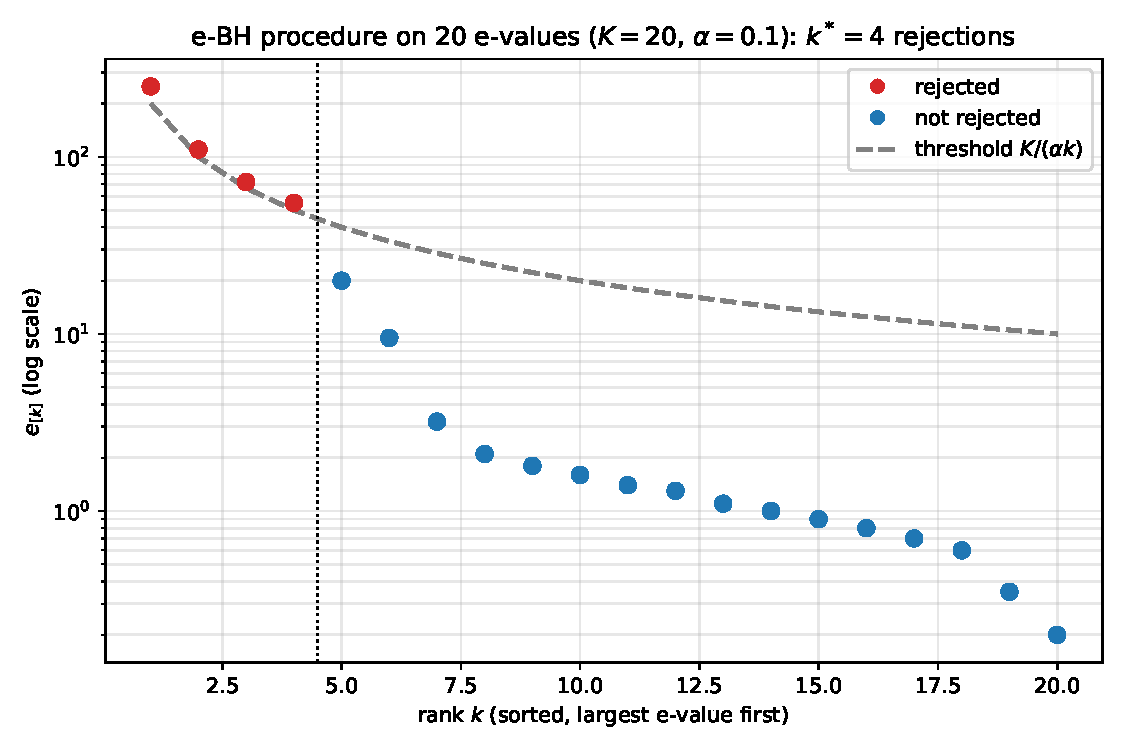
\includegraphics[width=0.78\textwidth]{ebh_illustration.pdf}
\end{center}
\footnotesize Sorted e-values (largest first) versus the e-BH threshold curve $K/(\alpha k)$ on a toy set of 20 e-values with $K=20,\alpha=0.1$. Points above the dashed curve (red) are rejected; the vertical dotted line marks the cutoff $k^\ast=4$.
\end{frame}

% ============================================================
\begin{frame}[fragile]{Python: the e-BH procedure on our 10 coins}
\begin{lstlisting}[language=Python]
import numpy as np

e = np.array([0.6, 12.0, 0.4, 34.0, 0.8,
              90.0, 0.5, 200.0, 24.0, 0.7])
coins = [f"Coin {i+1}" for i in range(10)]
K, alpha = len(e), 0.1

order = np.argsort(-e)          # sort descending
e_sorted = e[order]
k_idx = np.arange(1, K + 1)

# e-BH: k* = max{ k : k * e_[k] / K >= 1/alpha }
satisfies = (k_idx * e_sorted / K) >= (1 / alpha)
k_star = np.max(np.where(satisfies)[0]) + 1 if satisfies.any() else 0

rejected = [coins[i] for i in order[:k_star]]
print("Sorted e-values:", e_sorted)
print("k* =", k_star)
print("Rejected hypotheses:", rejected)

# --- output ---
# Sorted e-values: [200.  90.  34.  24.  12.   0.8  0.7  0.6  0.5  0.4]
# k* = 3
# Rejected hypotheses: ['Coin 8', 'Coin 6', 'Coin 4']
\end{lstlisting}
\end{frame}

% ============================================================
\begin{frame}[allowframebreaks]{Why e-BH controls the FDR: self-consistency}

\textbf{Intuition.} We want to show that no matter how the compound e-values $E_1,\dots,E_K$ depend on each other, e-BH's FDR never exceeds $\alpha$. The key structural property of e-BH is that \emph{every rejected hypothesis has a big enough e-value, relative to the total number of rejections}. We isolate this property and show it alone is enough for FDR control -- this makes the proof apply to a whole family of related procedures at once (self-consistent ones), not just to e-BH.

\begin{block}{Definition 9.9: Self-consistent e-testing procedures}
An e-testing procedure $\mathcal{D}$ is \emph{self-consistent at level $\alpha$} if every rejected hypothesis $H_k$ has realized e-value satisfying
\[
e_k \ \ge\ \frac{K}{\alpha R_{\mathcal{D}}},
\]
where $R_\mathcal{D}=|\mathcal{D}|$ is the total number of rejections. The e-BH procedure is a special case (in fact the \emph{largest} self-consistent procedure: it dominates every other self-consistent procedure).
\end{block}
In words: if you reject $R_\mathcal{D}$ hypotheses total, each one better have an e-value of at least $K/(\alpha R_\mathcal{D})$ -- the more you reject, the higher a bar each individual rejection must clear (since the same total error budget $K$ is being spread over more discoveries with a laxer per-rejection threshold as $R_\mathcal D$ grows, this exactly balances out, as the proof below shows).

\framebreak

\begin{block}{Theorem 9.11: FDR control (and post-hoc FDR control)}
Any self-consistent e-testing procedure at level $\alpha$, including e-BH, has FDR at most $\alpha$, for \emph{any} $\mathbb{P}$ and \emph{any} compound e-variables, regardless of their dependence structure. In fact, for any family $(\mathcal{D}_\alpha)_{\alpha\in(0,1)}$ of self-consistent procedures indexed by level,
\[
\mathbb{E}^{\mathbb{P}}\Big[\sup_{\alpha\in(0,1)} \frac{F_{\mathcal{D}_\alpha}}{\alpha R_{\mathcal{D}_\alpha}}\Big] \le 1,
\]
a \emph{post-hoc} guarantee valid even if $\alpha$ itself is chosen after looking at the data. If $E_1,\dots,E_K$ happen to be ordinary e-variables (not just compound), the bound improves to $K_0/K$.
\end{block}

\framebreak

\textbf{Step-by-step proof walkthrough.} Let $\mathbf{E}=(E_1,\dots,E_K)$ be arbitrary compound e-variables, and $\mathcal{D}_\alpha(\mathbf{E})$ the rejection set.

\begin{enumerate}
\item \textbf{Rewrite the FDP} using indicators: for the true-null set $\Nc$,
\[
\frac{F_{\mathcal{D}_\alpha}}{\alpha R_{\mathcal{D}_\alpha}} = \frac{|\mathcal{D}_\alpha(\mathbf{E})\cap\Nc|}{\alpha(R_{\mathcal{D}_\alpha}\vee 1)} = \sum_{k\in\Nc} \frac{\mathbb{1}\{k\in\mathcal{D}_\alpha(\mathbf{E})\}}{\alpha(R_{\mathcal{D}_\alpha}\vee 1)}.
\]
\item \textbf{Bound each surviving term by self-consistency:} if $k \in \mathcal{D}_\alpha(\mathbf{E})$ (i.e., $H_k$ was rejected), self-consistency says $E_k \ge K/(\alpha R_{\mathcal{D}_\alpha})$, i.e., $\frac{1}{\alpha (R_{\mathcal{D}_\alpha}\vee 1)} \le \frac{E_k}{K}$. Substituting,
\[
\frac{F_{\mathcal{D}_\alpha}}{\alpha R_{\mathcal{D}_\alpha}} \ \le\ \sum_{k\in\Nc} \frac{\mathbb{1}\{k\in\mathcal{D}_\alpha(\mathbf{E})\}\, E_k}{K} \ \le\ \sum_{k\in\Nc} \frac{E_k}{K}.
\]
(The last step just drops the indicator, which can only increase the sum since $E_k\ge0$.)
\item \textbf{Take expectations and invoke the compound e-value bound:} by Definition 9.1, $\sum_{k\in\Nc}\mathbb{E}^{\mathbb{P}}[E_k] \le K$, so
\[
\mathbb{E}^{\mathbb{P}}\Big[\sup_{\alpha}\frac{F_{\mathcal{D}_\alpha}}{\alpha R_{\mathcal{D}_\alpha}}\Big] \le \mathbb{E}^{\mathbb{P}}\Big[\sum_{k\in\Nc}\frac{E_k}{K}\Big] \le 1.
\]
\item \textbf{Drop the supremum} over $\alpha$ (keeping only a single fixed $\alpha$) to recover the plain FDR bound: $\text{FDR}_{\mathcal{D}_\alpha} \le \alpha$.
\end{enumerate}
Notice that the whole argument never used independence, or any dependence assumption at all, among $E_1,\dots,E_K$ -- this is exactly why e-BH is dependence-robust.

\end{frame}

% ============================================================
\begin{frame}[allowframebreaks]{9.1.3 Boosting e-values with distributional information}

\textbf{Intuition.} e-BH as defined only ever uses each e-value in a very coarse way: it only matters whether $e_k$ clears certain grid thresholds $K/(\alpha k)$. If we know more about the null distribution of $E_k$, we can sometimes replace $E_k$ by a strictly larger quantity $b_k E_k$ ($b_k \ge 1$, a ``boosting factor'') that \emph{still} behaves like a valid e-value at the thresholds e-BH cares about -- giving strictly more power for free.

\begin{block}{The truncation function and boosting condition}
Let $K/\Kc := \{K/k : k \in \Kc\}$ and define $T:[0,\infty]\to[0,K]$ by
\[
T(x) = \frac{K}{\lceil K/x \rceil}\, \mathbb{1}\{x \ge 1\}, \qquad T(\infty)=K,
\]
i.e. $T$ rounds $x$ down to the nearest value in $K/\Kc \cup \{0\}$. A \emph{boosting factor} $b_k \ge 1$ for hypothesis $k$ must satisfy
\[
\mathbb{E}^{\mathbb{P}}[T(\alpha b_k E_k)] \le \alpha \qquad \text{for } \mathbb{P}\in\mathcal{P}_k. \tag{9.2}
\]
The \emph{boosted e-value} is $E_k' = b_k E_k$. Choosing $b_k=1$ always works (since $T(x)\le x$), but the goal is to find the \emph{largest} valid $b_k$, which requires distributional knowledge of $E_k$ under the null; with no such knowledge, $b_k=1$ is forced.
\end{block}

\framebreak

\begin{block}{Theorem 9.13}
Applied to arbitrary nonnegative $E_1',\dots,E_K'$, the e-BH procedure at level $\alpha$ satisfies
\[
\mathbb{E}^{\mathbb{P}}\Big[\frac{F_\mathcal{D}}{R_\mathcal{D}}\Big] \ \le\ \frac{1}{K}\sum_{k\in\Nc}\mathbb{E}^{\mathbb{P}}[T(\alpha E_k')].
\]
In particular, if $E_1',\dots,E_K'$ are the boosted e-values from (9.2), FDR is controlled at level $K_0\alpha/K \le \alpha$.
\end{block}

\textbf{Intuition for why this works.} Since e-BH only ever rejects at the grid thresholds $K/(\alpha k)$, replacing each $e_k$ with $T(\alpha e_k)/\alpha$ (i.e., rounding it down to the nearest relevant grid level) produces the \emph{exact same rejection set}. So it suffices that the \emph{rounded-down} version of $\alpha E_k$ behaves like a bona fide e-value, which is precisely condition (9.2). We can boost individual e-values this way, or boost jointly across a whole compound e-value collection using boosting factors satisfying the analogous pooled condition $\sum_{k:\mathbb{P}\in\mathcal{P}_k}\mathbb{E}^{\mathbb{P}}[T(\alpha b_k E_k)] \le K\alpha$.

\end{frame}

% ============================================================
\begin{frame}[allowframebreaks]{9.1.4 Connection between e-BH and BH}

\textbf{Intuition.} P-values and e-values are related by $P_k = 1/E_k$ (a valid e-value always gives a valid p-value this way). So it is natural to ask: is e-BH just BH in disguise? The answer is subtle: e-BH \emph{is} literally BH applied to $1/E_1,\dots,1/E_K$, but the FDR guarantee for plain BH normally needs an extra dependence assumption (PRDS or independence) that e-BH does not need.

\begin{block}{Definition 9.14: The BH and BHY procedures}
With p-values $p_1\le\dots\le p_K$ sorted ascending, BH at level $\alpha$ rejects the $k^\ast$ smallest, where $k^\ast = \max\{k : Kp_{(k)}/k \le \alpha\}$. The \emph{BHY} procedure (Benjamini--Yekutieli correction) applies BH to $\ell_K p_1,\dots,\ell_K p_K$ instead, where $\ell_K = \sum_{k=1}^K 1/k \approx \log K$.
\end{block}

\begin{block}{Definition 9.15: PRDS (positive regression dependence on a subset)}
A set $A\subseteq\mathbb{R}^K$ is \emph{increasing} if $\mathbf{x}\in A, \mathbf{y}\ge\mathbf{x} \Rightarrow \mathbf{y}\in A$. $(P_1,\dots,P_K)$ satisfies PRDS if for every null index $k$ and increasing set $A$, $x\mapsto\mathbb{P}\{(P_\ell)_{\ell\in\Kc}\in A \mid P_k\le x\}$ is increasing on $[0,1]$. (Informally: conditioning on a null p-value being small should not make other p-values look larger -- a positive-dependence condition, often hard to verify in practice.)
\end{block}

\framebreak

\textbf{Classical facts.} (i) BHY controls FDR at level $(K_0/K)\alpha$ under \emph{arbitrary} dependence. (ii) Plain BH controls FDR at level $(K_0/K)\alpha$ \emph{if} the p-values are independent or PRDS. The price for full dependence-robustness (BHY) is the extra factor $\ell_K \approx \log K$, which shrinks all p-values, and hence typically causes many fewer rejections.

\begin{block}{Proposition 9.16 and the e-value viewpoint}
Since $P_k = 1/E_k$ is always a p-value when $E_k$ is an e-value, e-BH is \emph{exactly} BH applied to $1/E_1,\dots,1/E_K$ -- but e-BH's FDR guarantee (Theorem 9.11) needs no dependence assumption at all. Moreover, $f(p) = T(\alpha/(\ell_K p))/\alpha$ is a valid \emph{calibrator} (turns a p-value into an e-value), and the BHY procedure equals e-BH applied to the calibrated e-values $f(P_1),\dots,f(P_K)$.
\end{block}

\textbf{Takeaway.} e-BH quietly \emph{contains} both BH (as a special "boosted e-values" instance, using knowledge of PRDS to construct the boost) and BHY (via the calibrator $f$) as special cases -- this is a first hint of the universality theme of Section 9.2.

\end{frame}

% ============================================================
\section{9.2 Universality of compound e-values and e-BH}
% ============================================================

\begin{frame}[allowframebreaks]{9.2: Every FDR procedure secretly is e-BH}

\textbf{Intuition.} This is one of the more surprising results in the chapter: \emph{any} procedure that controls FDR -- no matter how it was built, whether it uses e-values, p-values, or something else entirely -- can be re-expressed as ``run e-BH on some cleverly chosen compound e-values.'' This does not mean every procedure was secretly designed with e-values in mind; it means the e-BH template is rich enough to represent every valid FDR procedure after the fact.

\begin{block}{Theorem 9.18: From FDR control to compound e-values}
Let $\mathcal{D}$ be any procedure controlling FDR at level $\alpha$. Let $V_k \in \{0,1\}$ indicate whether $\mathcal{D}$ rejects $H_k$ (so $F_\mathcal{D}=\sum_{k\in\Nc}V_k$, $R_\mathcal{D}=\sum_{k\in\Kc}V_k$). Define
\[
E_k = \frac{K}{\alpha}\cdot\frac{V_k}{R_\mathcal{D}\vee 1}. \tag{9.3}
\]
Then $E_1,\dots,E_K$ are compound e-variables for $(\mathcal{P}_1,\dots,\mathcal{P}_K)$.
\end{block}

\textbf{Why:} $\sum_{k:\mathbb{P}\in\mathcal{P}_k}\mathbb{E}^{\mathbb{P}}[E_k] = \frac{K}{\alpha}\mathbb{E}^{\mathbb{P}}\big[\frac{F_\mathcal{D}}{R_\mathcal{D}\vee1}\big] \le \frac{K}{\alpha}\cdot\alpha = K$, using exactly the FDR guarantee of $\mathcal{D}$.

\framebreak

\begin{block}{Theorem 9.19: Universality of e-BH}
Let $\mathcal{D}$ be any FDR-controlling procedure at level $\alpha$. Then there exist compound e-values such that e-BH applied to them makes \emph{exactly} the same discoveries as $\mathcal{D}$. Further, if $\mathcal{D}$ is \emph{admissible} (cannot be enlarged while still controlling FDR), these compound e-values can be chosen to be \emph{tight}.
\end{block}
The proof takes the $E_k$'s from (9.3) and, if they are not already tight (i.e. $K^\ast := \sup_{\mathbb{P}}\sum_{k:\mathbb{P}\in\mathcal{P}_k}\mathbb{E}^{\mathbb{P}}[E_k] < K$), rescales them by $K/K^\ast$ to use up the full budget; admissibility then forces the rescaled e-BH procedure to coincide with $\mathcal{D}$ itself (otherwise it would strictly dominate $\mathcal{D}$, contradicting admissibility).

\framebreak

\textbf{A practical payoff: combining and derandomizing procedures.} Suppose $L$ different multiple-testing procedures $\mathcal{D}_1,\dots,\mathcal{D}_L$ are run (perhaps by different teams, using different methods, each controlling FDR at its own level $\alpha_\ell$), and we want to merge them into a single procedure. Recipe:

\begin{enumerate}
\item For each procedure $\ell$, form compound e-variables $E_1^{(\ell)},\dots,E_K^{(\ell)}$ via Theorem 9.18 (this always exists).
\item Fix convex weights $w_1,\dots,w_L\ge0$, $\sum_\ell w_\ell=1$ (possibly random, but independent of the e-values), and combine via Example 9.4: $E_k = \sum_{\ell=1}^L w_\ell E_k^{(\ell)}$.
\item Apply e-BH at level $\alpha$ to the combined $E_1,\dots,E_K$.
\end{enumerate}
This combined procedure controls FDR at level $\alpha$ -- and the original levels $\alpha_\ell$ do not even matter for the final guarantee! A key application is \emph{derandomization}: if $\mathcal{D}_\ell$ depends on external randomness $U_\ell$, averaging over many independent copies (as $L\to\infty$) removes the procedure's sensitivity to the random seed while still controlling FDR.

\end{frame}

% ============================================================
\section{9.3 Log-optimal simple separable compound e-values}
% ============================================================

\begin{frame}[allowframebreaks]{9.3: Motivation and Robbins' compound decision theory}

\textbf{Intuition.} So far we assumed compound e-values are handed to us. Section 9.3 asks: in a clean sequence model where each hypothesis $k$ has its own data point $X_k$, what is the \emph{best possible} compound e-value we could construct, if we are only allowed the simplest possible rule -- apply the \emph{same} function $f$ to each $X_k$? This connects directly to a classical idea in statistics: Robbins' compound decision theory.

\begin{block}{Definition 9.20: Simple separable e-variables}
$E_1,\dots,E_K$ are \emph{separable} if $E_k = E_k(X_k)$ depends only on the $k$-th coordinate of the data. They are \emph{simple separable} if, further, $E_k = f(X_k)$ for the \emph{same} function $f$ across all $k$.
\end{block}

\textbf{Background (9.3.1): Robbins' compound decision problem.} In the Gaussian sequence model, $X_k \sim N(\mu_k,1)$ independently, $k\in\Kc$, with unknown means $\boldsymbol\mu=(\mu_1,\dots,\mu_K)$ fixed. We want estimators $\hat\mu_k$ minimizing the \emph{compound} (averaged) risk $\frac{1}{K}\sum_k \mathbb{E}^{\boldsymbol\mu}[(\hat\mu_k-\mu_k)^2]$.

\framebreak

\textbf{The fundamental theorem of compound decisions.} Let $M = \frac{1}{K}\sum_k \delta_{\mu_k}$ be the empirical distribution of the true means (a single ``prior''), and consider the associated univariate Bayes problem $\mu'\sim M,\ X'\mid\mu' \sim N(\mu',1)$. For \emph{any} fixed function $s:\mathbb{R}\to\mathbb{R}$,
\[
\frac{1}{K}\sum_{k\in\Kc}\mathbb{E}^{\boldsymbol\mu}[(s(X_k)-\mu_k)^2] = \mathbb{E}^{\mathbb{P}_M}[(s(X')-\mu')^2].
\]
So the best \emph{simple separable} estimator $s$ (same function applied to every $X_k$) is exactly the Bayes estimator under $M$: $s(x) = \mathbb{E}^{\mathbb{P}_M}[\mu' \mid X'=x]$. This gives an oracle benchmark: even though the oracle needs to know the true $\boldsymbol\mu$ (through $M$) to construct $s$, it is still constrained to use the \emph{same} $s$ for every coordinate -- exactly like our compound e-value problem, where the oracle also ``knows everything'' but the estimator/e-value function itself must be simple and separable.

\framebreak

\textbf{9.3.2: The log-optimal simple separable compound e-value.} Suppose each null $\mathcal{P}_k=\{\mathbb{S} : \mathbb{S}_k=\mathbb{P}_k\}$ is a simple point null on the $k$-th marginal, with $d\nu$-density $p_k$, and suppose alternatives $\mathbb{Q}_k$ have densities $q_k$. We seek the simple separable function $s$ maximizing the \emph{compound expected log-wealth} (a natural notion of power for e-values):
\[
\underset{s:\mathcal{Y}\to[0,\infty)}{\text{maximize}} \quad \frac{1}{K}\sum_{k\in\Kc} \mathbb{E}^{\mathbb{Q}_k}[\log(s(X_k))] \quad \text{s.t. } s(X_1),\dots,s(X_K) \text{ are compound e-variables.} \tag{9.8}
\]

\begin{block}{Theorem 9.21: Log-optimal simple separable compound e-values}
The optimal solution to (9.8) is the likelihood ratio of the \emph{mixtures}:
\[
s(x) = \frac{\sum_{j\in\Kc} q_j(x)}{\sum_{j\in\Kc} p_j(x)}.
\]
\end{block}
\textbf{Intuition for the proof:} averaging both the objective and the compound e-value constraint over $k\in\Kc$ turns the whole compound problem into a single ordinary e-value optimization problem (of the type solved in Chapter 3) for testing the average null density $\bar p = \frac1K\sum_j p_j$ against the average alternative density $\bar q = \frac1K\sum_j q_j$; the log-optimal single e-value there is exactly the likelihood ratio $\bar q(x)/\bar p(x) = s(x)$.

\framebreak

\begin{block}{Proposition 9.22: Tight simple separable compound e-values must look like this}
If $E_1,\dots,E_K$ are \emph{tight} simple separable compound e-values, then there exist $d\nu$-densities $q_1,\dots,q_K$ such that $E_k$ has the form of Theorem 9.21 on the support of $\bar p=\frac1K\sum_k p_k$, and (without loss of generality) one may take $q_1=\cdots=q_K$.
\end{block}

\textbf{Why should we care?} The optimal compound e-value $s(x)=\bar q(x)/\bar p(x)$ requires knowing $q_1,\dots,q_K$ (the true alternatives) -- information we rarely have exactly. But if $K$ is large and all the alternatives share a common unknown structure (e.g., a shared nuisance parameter $\theta$), we may be able to \emph{learn} that shared structure by pooling data across all $K$ hypotheses (empirical Bayes / compound decision theory), even though we could never learn it from a single hypothesis's data alone. This is the deep reason ``compound'' e-values, which allow such pooling, can outperform naive per-hypothesis e-values when $K$ is large.

\end{frame}

% ============================================================
\begin{frame}[fragile]{Python: log-optimal separable compound e-value (Gaussian model)}
\begin{lstlisting}[language=Python]
import numpy as np
rng = np.random.default_rng(1)

# Gaussian sequence model: H_k : X_k ~ N(0,1) (null); K=10 hypotheses.
# Suppose (from pooling data / domain knowledge) we believe the
# alternative means are mu = (0,...,0, 2, 2.5, 3, 3.5) (last 4 biased).
K = 10
mu = np.array([0,0,0,0,0,0, 2.0, 2.5, 3.0, 3.5])

def p_dens(x):            # common null density N(0,1)
    return np.exp(-0.5*x**2)/np.sqrt(2*np.pi)

def q_mix(x):              # mixture of alternative densities
    return np.mean([np.exp(-0.5*(x-m)**2)/np.sqrt(2*np.pi) for m in mu], axis=0)

def s(x):                  # log-optimal simple separable e-value, Thm 9.21
    return q_mix(x) / p_dens(x)

# Monte Carlo check: under the GLOBAL null (all mu=0), E[s(X_k)] <= 1 each,
# and the K-fold sum should not exceed K (the compound e-value budget).
n_mc = 200_000
vals = [np.mean(s(rng.normal(0, 1, n_mc))) for _ in range(K)]
print("E[s(X_k)] per hypothesis:", np.round(vals, 3))
print("Sum over all k:", round(sum(vals), 2), " (budget: K =", K, ")")

# --- output (Monte Carlo, matches theory up to sampling error) ---
# E[s(X_k)] per hypothesis: [0.985 1.061 0.99  0.991 1.009 0.994 1.057 0.99  1.002 0.983]
# Sum over all k: 10.06  (budget: K = 10)
\end{lstlisting}
\end{frame}

% ============================================================
\section{9.4 A minimally adaptive e-BH procedure}
% ============================================================

\begin{frame}[allowframebreaks]{9.4: Getting one more rejection almost for free}

\textbf{Intuition.} e-BH is sometimes needlessly conservative for small $K$. The fix here costs almost nothing: first spend a tiny sliver of the error budget testing the \emph{global null} (``are all $K$ hypotheses simultaneously true?''); if that global null is confidently rejected, we know \emph{at least one} hypothesis is false, so we can afford to run e-BH slightly more aggressively (at a laxer level $\alpha'>\alpha$) on the rest, since one ``guaranteed'' true rejection is already banked.

\begin{block}{The minimally adaptive e-BH procedure $\mathcal{D}_\alpha^F$}
Fix an e-merging function $F:[0,\infty)^K\to[0,\infty)$ (Chapter 8) -- e.g. the arithmetic mean $\mathbb{M}_K(e_1,\dots,e_K)=\frac1K\sum_k e_k$. Given realized e-values $e_1,\dots,e_K$ and level $\alpha$:
\begin{enumerate}
\item[\textbf{Step 1.}] Test the global null $\bigcap_{k=1}^K \mathcal{P}_k$: reject it if $F(e_1,\dots,e_K)\ge 1/\alpha$.
\item[\textbf{Step 2.}] If the global null is \emph{not} rejected, output $\mathcal{D}_\alpha^F=\emptyset$ (no discoveries).
\item[\textbf{Step 3.}] If the global null \emph{is} rejected, run the ordinary e-BH procedure at the slightly larger level $\alpha' = K\alpha/(K-1)$, and output its rejection set.
\end{enumerate}
\end{block}

\framebreak

\begin{block}{Proposition 9.23}
For any $\alpha\in(0,1)$, the improved procedure $\mathcal{D}_\alpha^F$ applied to arbitrary e-values has FDR at most $\alpha$. Moreover, taking $F=\mathbb{M}_K$ (the arithmetic mean) makes $\mathcal{D}_\alpha^{\mathbb{M}_K}$ \emph{dominate} plain e-BH: $\mathcal{D}_\alpha \subseteq \mathcal{D}_\alpha^{\mathbb{M}_K}$ always.
\end{block}

\textbf{Why FDR is still controlled (sketch).} If not all nulls are true ($K_0<K$), Theorem 9.11 applied at the larger level $\alpha'=K\alpha/(K-1)$ already gives FDR $\le (K_0/K)\alpha' \le \alpha$. If instead \emph{all} hypotheses are truly null ($K_0=K$), the only way to make any discovery at all is to (falsely) reject the global null, which by Markov's inequality happens with probability at most $\alpha$ -- so FDR $\le \alpha$ in this case too. Either way, $\alpha$ is never exceeded.

\framebreak

\textbf{Running example, continued: minimally adaptive e-BH on our 10 coins.}
\textbf{Step 1: test the global null.} Using $F=\mathbb{M}_K$ (arithmetic mean):
\[
\bar e = \frac{0.6+12.0+0.4+34.0+0.8+90.0+0.5+200.0+24.0+0.7}{10} = \frac{352.2}{10} = 35.22.
\]
Compare to $1/\alpha = 1/0.1 = 10$: since $35.22 \ge 10$, the global null is \textbf{rejected}.

\textbf{Step 2: recompute at the laxer level.}
\[
\alpha' = \frac{K\alpha}{K-1} = \frac{10 \times 0.1}{9} = \frac{1}{9} \approx 0.1111, \qquad \frac{K}{\alpha'} = \frac{10}{1/9} = 90.
\]

\framebreak

\textbf{Step 3: re-run e-BH's threshold check at the new bar of 90 (instead of 100).}
\[
\begin{array}{c|c|c}
k & e_{[k]} & k\cdot e_{[k]} \text{ vs. } 90\\
\hline
1 & 200.0 & 200.0 \ge 90 \ \checkmark\\
2 & 90.0 & 180.0 \ge 90 \ \checkmark\\
3 & 34.0 & 102.0 \ge 90 \ \checkmark\\
4 & 24.0 & 96.0 \ \ge 90 \ \checkmark \ \textbf{(newly passes!)}\\
5 & 12.0 & 60.0 < 90 \ \times
\end{array}
\]
Now $k^\ast = 4$: minimally adaptive e-BH rejects coins $8,6,4,9$ -- \textbf{one more discovery (coin 9) than plain e-BH}, which only rejected coins $8,6,4$. This single extra global-null test, essentially free, recovered the near-miss we flagged earlier!

\end{frame}

% ============================================================
\begin{frame}[fragile]{Python: minimally adaptive e-BH on our 10 coins}
\begin{lstlisting}[language=Python]
import numpy as np

e = np.array([0.6, 12.0, 0.4, 34.0, 0.8,
              90.0, 0.5, 200.0, 24.0, 0.7])
coins = [f"Coin {i+1}" for i in range(10)]
K, alpha = len(e), 0.1

def ebh_kstar(e_arr, lvl):
    order = np.argsort(-e_arr)
    e_sorted = e_arr[order]
    k_idx = np.arange(1, len(e_arr) + 1)
    sat = (k_idx * e_sorted / len(e_arr)) >= (1 / lvl)
    k = np.max(np.where(sat)[0]) + 1 if sat.any() else 0
    return k, order

# Step 1: global null test via the arithmetic mean e-merging function
mean_e = e.mean()
print("Global-null e-value (mean):", mean_e, " vs 1/alpha =", 1/alpha)

if mean_e >= 1 / alpha:
    alpha_prime = K * alpha / (K - 1)          # Step 3: laxer level
    k_star, order = ebh_kstar(e, alpha_prime)
else:
    k_star, order = 0, np.argsort(-e)          # Step 2: no discoveries

print("alpha' =", round(alpha_prime, 4))
print("k*_adaptive =", k_star,
      "rejected:", [coins[i] for i in order[:k_star]])

# --- output ---
# Global-null e-value (mean): 35.22  vs 1/alpha = 10.0
# alpha' = 0.1111
# k*_adaptive = 4 rejected: ['Coin 8', 'Coin 6', 'Coin 4', 'Coin 9']
\end{lstlisting}
\end{frame}

% ============================================================
\begin{frame}[allowframebreaks]{9.4, continued: boosting inside the adaptive procedure}

\textbf{Intuition.} The minimally adaptive idea composes cleanly with the boosting idea from Section 9.1.3: boost the raw e-values first (using distributional knowledge), then run the adaptive two-step test on the boosted values.

\begin{block}{Minimally adaptive e-BH with boosted e-values}
\begin{enumerate}
\item Boost the raw e-values at level $\alpha$, obtaining $e_1',\dots,e_K'$ via (9.2).
\item If $S(e_1',\dots,e_K') < 1/\alpha$ (where $S(e_1,\dots,e_K):=\max_k \frac{k e_{[k]}}{K}$), return $\emptyset$.
\item Otherwise, re-boost the raw e-values at the laxer level $\alpha'=K\alpha/(K-1)$.
\item Return the discoveries of ordinary e-BH applied to the re-boosted e-values from Step 3.
\end{enumerate}
\end{block}

\textbf{Why use $S$ instead of the mean in Step 2?} The function $S(e_1,\dots,e_K)=\max_k \frac{k e_{[k]}}{K}$ is itself an e-merging function, and it is \emph{dominated} by the arithmetic mean $\mathbb{M}_K$ (since $\sum_{k=1}^K e_k \ge k\, e_{[k]}$ for every $k$ -- the sum of all values is at least $k$ times the $k$-th largest). Crucially, boosted e-values need not remain valid e-values after arithmetic averaging, so we instead use $S$, whose global-null test is exactly equivalent to ``e-BH makes at least one rejection.'' This variant again dominates plain e-BH and controls FDR at level $\alpha$, by the same argument as Proposition 9.23.

\end{frame}

% ============================================================
\section{9.5 Stochastic rounding of e-values and randomized e-BH}
% ============================================================

\begin{frame}[allowframebreaks]{9.5: Turning wasted precision into power via randomization}

\textbf{Intuition.} e-BH only ever cares whether $e_k$ crosses certain grid thresholds $K/(\alpha k)$. If an e-value sits \emph{strictly between} two grid points, rounding it \emph{down} to the lower grid point changes nothing about e-BH's decision -- but rounding it \emph{up} could push a near-miss over the edge. The catch: rounding up would inflate the expectation, breaking the e-value property. The resolution: round up \emph{or} down \emph{randomly}, with probabilities chosen so the expectation is exactly preserved. This costs nothing in expectation, but gives a chance (not a certainty) of extra power.

\begin{block}{Stochastic rounding onto a grid}
Let $\mathcal{G}\subseteq[0,\infty]$ be closed, $g_\ast=\inf\mathcal{G}$, $g^\ast=\sup\mathcal{G}$. For $x\in[g_\ast,g^\ast]$, let $x^+ = \inf\{y\in\mathcal{G}:y\ge x\}$ and $x_- = \sup\{y\in\mathcal{G}:y\le x\}$. Define
\[
S_{\mathcal{G}}(x) = \begin{cases} x_- & \text{w.p. } \dfrac{x^+-x}{x^+-x_-}, \\[4pt] x^+ & \text{w.p. } \dfrac{x-x_-}{x^+-x_-}, \end{cases}
\]
and $S_{\mathcal{G}}(x)=x$ if $x<g_\ast$, $x>g^\ast$, $x\in\mathcal{G}$, or $x^+=\infty$.
\end{block}

\framebreak

\begin{block}{Proposition 9.24}
For any grid $\mathcal{G}$ and integrable $X$, $\mathbb{E}^{\mathbb{P}}[X] = \mathbb{E}^{\mathbb{P}}[S_\mathcal{G}(X)]$. In particular, if $X$ is an e-variable, so is $S_\mathcal{G}(X)$.
\end{block}
\textbf{Why:} by construction $\mathbb{E}[S_\mathcal{G}(x)] = x\cdot\frac{x^+-x}{x^+-x_-}\cdot 0^\circ \dots$ -- more precisely, a short calculation shows $\mathbb{E}[S_\mathcal{G}(x)\mid x]=x$ exactly for every real $x$, so applying $\mathbb{E}[\cdot]$ to any random $X$ leaves its mean unchanged. Crucially, $S_\mathcal{G}(X)$ can be \emph{larger} than $X$ with positive probability (whenever it rounds up), even though its expectation cannot increase -- this is the whole source of the extra power.

\framebreak

\textbf{Applying this to e-BH.} Fix $\alpha$ and let $\mathcal{G}_\alpha = \{K/(\alpha k) : k\in\Kc\}\cup\{0,\infty\}$ -- exactly the grid of thresholds e-BH cares about.

\begin{block}{Definition: Ge-BH, De-BH, Ue-BH}
\begin{itemize}
\item \textbf{Ge-BH} (grid-rounded e-BH): apply e-BH to $S_{\mathcal{G}_\alpha}(E_1),\dots,S_{\mathcal{G}_\alpha}(E_K)$.
\item \textbf{De-BH} (doubly-rounded e-BH, Algorithm 9.28): apply e-BH to the once-rounded values; let $k^\ast$ be its number of rejections and set $\hat\alpha^\ast = \alpha(k^\ast+1)/K$; then reject $H_i$ if $S_{\hat\alpha^{\ast}}(S_{\mathcal{G}_\alpha}(E_i)) \ge (\hat\alpha^\ast)^{-1}$ (a second round of rounding onto the data-dependent grid $\{0,(\hat\alpha^\ast)^{-1},\infty\}$).
\item \textbf{Ue-BH} (uniformly-randomized e-BH): apply e-BH to $E_1/U,\dots,E_K/U$ for an independent $U\sim\text{Unif}[0,1]$.
\end{itemize}
\end{block}

\framebreak

\begin{block}{Theorems 9.27 and 9.29}
For arbitrarily dependent e-values, Ge-BH controls FDR $\le \alpha$ and its discovery set is always a superset of e-BH's. Moreover, $\mathbb{P}(\mathcal{D}_{\text{GeBH}} \supsetneq \mathcal{D}_{\text{eBH}}) > 0$ under a mild condition (satisfied e.g. whenever the e-values are continuously distributed). De-BH and Ue-BH further enlarge the discovery set (De-BH $\supseteq$ Ge-BH $\supseteq$ eBH; Ue-BH $\supseteq$ eBH), while still controlling FDR $\le \alpha$.
\end{block}

\textbf{A note on randomization.} It is \emph{not} obvious, in general, that randomizing a procedure should help. The authors conjecture that BH itself (with p-values, under positive dependence) cannot be improved by randomization without sacrificing power elsewhere -- but for e-BH, stochastic rounding genuinely helps, essentially because e-values, unlike p-values, are continuous-valued quantities whose exact magnitude (not just whether they cross one threshold) carries usable information.

\end{frame}

% ============================================================
\begin{frame}[allowframebreaks]{Running example, continued: randomized e-BH (Ge-BH)}

\textbf{Step 1: build the grid.} With $K=10,\alpha=0.1$: $\mathcal{G}_\alpha = \{100, 50, 33.33, 25, 20, 16.67, 14.29, 12.5, 11.11, 10\}\cup\{0,\infty\}$ (the values $K/(\alpha k)$ for $k=1,\dots,10$).

\textbf{Step 2: stochastically round each coin's e-value onto $\mathcal{G}_\alpha$.} For example, coin 9's e-value $24.0$ sits between grid points $20$ and $25$; it rounds up to $25$ with probability $\frac{24-20}{25-20}=0.8$ and down to $20$ with probability $0.2$. Similarly coin 2's e-value $12.0$ sits between $11.11$ and $12.5$, rounding up with probability $\frac{12-11.11}{12.5-11.11}\approx0.64$.

\textbf{Step 3: re-run e-BH on the rounded values.} Using a fixed random seed for reproducibility, one realization gives:
\[
\text{rounded } e\text{-values} = (0,\ 12.5,\ 0,\ 50,\ 0,\ 50,\ 0,\ 200,\ 25,\ 0)
\]
(coins 1,3,5,7,10, whose original e-values were all below the smallest grid point 10, round down to 0 or up to 10 depending on the draw; here they all rounded to 0). Re-checking the threshold ($k\cdot e_{[k]} \ge 100$): ranks $1$--$4$ ($200, 50, 50, 25$) give $200, 100, 150, 100$ -- all $\ge 100$. So $k^\ast=4$: Ge-BH rejects coins $8, 4, 6, 9$, again recovering the extra rejection of coin 9 -- this time through genuine randomization rather than adaptivity, and this happens with probability roughly $80\%$ over the randomness of the rounding (verified by repeating this simulation many times).

\end{frame}

% ============================================================
\begin{frame}[fragile]{Python: stochastic rounding and randomized e-BH (Ge-BH)}
\begin{lstlisting}[language=Python]
import numpy as np
rng = np.random.default_rng(0)

e = np.array([0.6, 12.0, 0.4, 34.0, 0.8,
              90.0, 0.5, 200.0, 24.0, 0.7])
coins = [f"Coin {i+1}" for i in range(10)]
K, alpha = len(e), 0.1

grid = np.sort([K/(alpha*k) for k in range(1, K+1)] + [0.0])  # G_alpha (finite part)

def stochastic_round(x, rng):
    if x <= 0 or x in grid:
        return x
    below, above = grid[grid <= x], grid[grid >= x]
    if len(above) == 0:        # x above top grid point -> x^+ = infinity
        return x
    x_minus, x_plus = below.max(), above.min()
    if x_plus == x_minus:
        return x
    p_up = (x - x_minus) / (x_plus - x_minus)
    return x_plus if rng.random() < p_up else x_minus

def ebh_kstar(e_arr, lvl):
    order = np.argsort(-e_arr)
    e_sorted = e_arr[order]
    k_idx = np.arange(1, len(e_arr) + 1)
    sat = (k_idx * e_sorted / len(e_arr)) >= (1/lvl) - 1e-9
    k = np.max(np.where(sat)[0]) + 1 if sat.any() else 0
    return k, order

rounded = np.array([stochastic_round(x, rng) for x in e])
k_star, order = ebh_kstar(rounded, alpha)
print("Rounded e-values:", np.round(rounded, 3))
print("Ge-BH k* =", k_star, "rejected:", [coins[i] for i in order[:k_star]])

# --- output ---
# Rounded e-values: [  0.   12.5   0.   50.    0.   50.    0.  200.   25.    0. ]
# Ge-BH k* = 4 rejected: ['Coin 8', 'Coin 4', 'Coin 6', 'Coin 9']
\end{lstlisting}
\end{frame}

% ============================================================
\begin{frame}{Numerical experiment: power gains from randomization}
\begin{center}
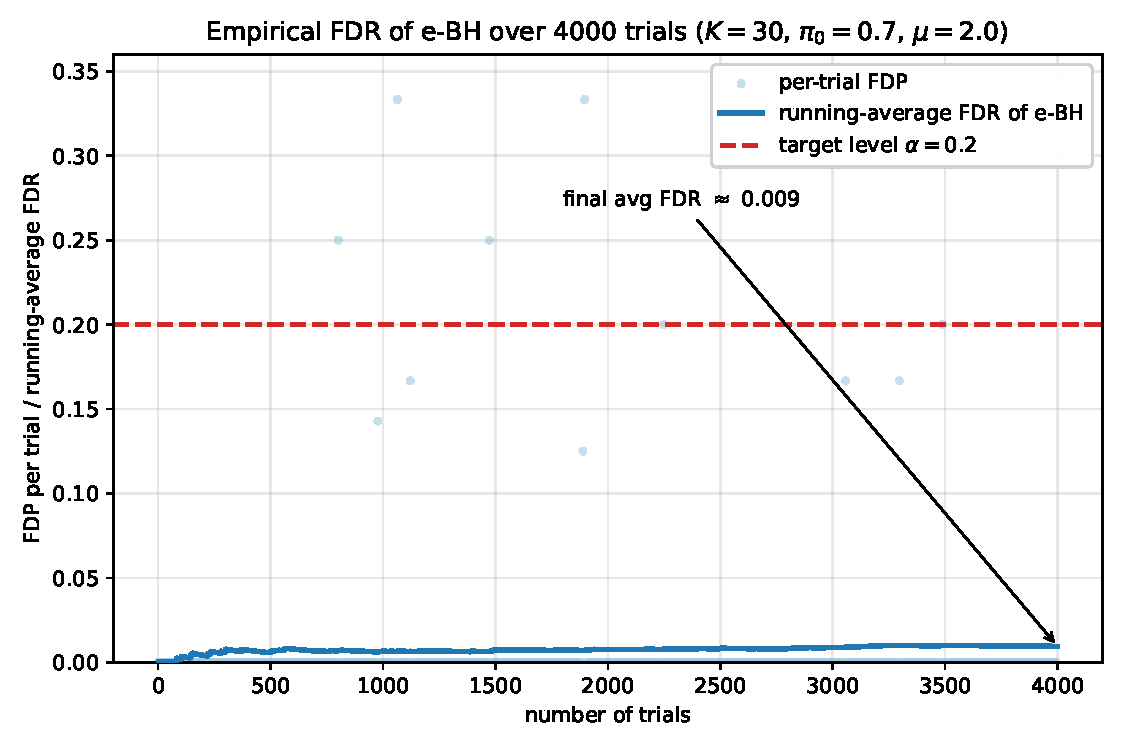
\includegraphics[width=0.62\textwidth]{fdr_simulation.pdf}
\end{center}
\footnotesize The book's own simulations (Figure 9.30, one-sided Gaussian testing, $K=100$, $\pi_0=0.3$) show that De-BH and Ue-BH can noticeably improve power over plain e-BH, especially under negative dependence between test statistics, while all three continue to control FDR at the nominal level -- exactly the phenomenon our own FDR simulation below re-creates in a simpler independent-samples setting.
\end{frame}

% ============================================================
\section{9.6 The closed e-BH procedure}
% ============================================================

\begin{frame}[allowframebreaks]{9.6: The closure principle for e-values}

\textbf{Intuition.} e-BH only ever uses one e-value per hypothesis. But if we could also test \emph{every combination} of hypotheses jointly (``are hypotheses 3, 7, and 9 \emph{all} true simultaneously?''), we could potentially justify rejecting a hypothesis whose individual e-value is unimpressive, as long as it belongs to enough jointly-rejectable groups. This is the classical \emph{closure principle} (well known for family-wise error rate control), now adapted to FDR and e-values.

\begin{block}{e-collections and the mean e-collection}
For $A\subseteq\Kc$, let $\mathcal{P}_A = \bigcap_{k\in A}\mathcal{P}_k$ (``all of $A$ are simultaneously null''). A family $\{E_A\}_{A\subseteq\Kc}$ is an \emph{e-collection} if $E_A$ is a genuine e-variable for $\mathcal{P}_A$, for every $A$ (with $E_\emptyset:=1$). If we only have one base e-value $E_k$ per hypothesis, the \emph{mean e-collection} is
\[
E_A = \frac{1}{|A|}\sum_{k\in A} E_k, \qquad A\subseteq\Kc.
\]
\end{block}

\begin{block}{The hypothetical FDP of a set $R$, relative to any candidate null set $A$}
\[
\text{FDP}_A(R) = \frac{|A\cap R|}{|R|\vee 1}.
\]
The \emph{true} FDP of a procedure that rejects $R$ is $\text{FDP}_{\Nc}(R)$, unknown since $\Nc$ is unknown -- $\text{FDP}_A(R)$ lets us reason about \emph{every possible} true-null configuration $A$ at once.
\end{block}

\framebreak

\begin{block}{Definition 9.31: The closed e-BH procedure}
Given an e-collection $\{E_A\}_{A\subseteq\Kc}$, define the \emph{candidate discovery sets}
\[
\mathcal{C}_\alpha = \Big\{ R\subseteq\Kc \,:\, E_A \ge \frac{\text{FDP}_A(R)}{\alpha} \ \text{ for all } A\subseteq\Kc \Big\}.
\]
The \emph{closed e-BH} procedure ($\overline{\text{e-BH}}$) rejects the \emph{largest} set $R\in\mathcal{C}_\alpha$ (breaking ties arbitrarily).
\end{block}
\textbf{Reading the condition.} $R\in\mathcal{C}_\alpha$ says: for every conceivable true-null set $A$, the pooled evidence against $A$ ($E_A$) is strong enough to justify the false-discovery proportion that $R$ \emph{would} have if $A$ were exactly the true nulls. Checking this for \emph{every} $A$ (not just $A=\Nc$, which we don't know) is what makes the guarantee unconditionally valid.

\framebreak

\begin{block}{Theorem 9.32}
Any procedure reporting some $R\in\mathcal{C}_\alpha$ (in particular closed e-BH) controls FDR at level $\alpha$, with the stronger post-hoc guarantee $\mathbb{E}^{\mathbb{P}}[\sup_\alpha\sup_{R\in\mathcal{C}_\alpha}\text{FDP}_{\Nc}(R)/\alpha]\le 1$. Moreover, with the mean e-collection, closed e-BH's rejection set is always a superset of \emph{both} plain e-BH's and the minimally adaptive e-BH's rejection sets: $\bar k \ge k^\sharp \ge k^\ast$.
\end{block}

\textbf{Step-by-step intuition for the proof.} Fix the true null set $A=\Nc$ (nonempty, else trivial). Every candidate $R\in\mathcal{C}_\alpha$ satisfies, \emph{by definition of $\mathcal{C}_\alpha$ applied at $A=\Nc$}, $\text{FDP}_{\Nc}(R)\le \alpha E_{\Nc}$. Since $E_\Nc$ is a genuine e-variable for $\mathcal{P}_\Nc$ (i.e. $\mathbb{E}^{\mathbb{P}}[E_\Nc]\le1$), taking expectations gives $\mathbb{E}^{\mathbb{P}}[\sup_R \text{FDP}_\Nc(R)/\alpha] \le \mathbb{E}^{\mathbb{P}}[E_\Nc]\le1$ -- FDR control follows immediately, \emph{without ever needing to know $\Nc$ itself}, because the definition of $\mathcal{C}_\alpha$ already baked in protection against every possible $A$, including the (unknown) true one.

\framebreak

\textbf{Running example, continued: closed e-BH on our 10 coins.} Using the mean e-collection $E_A = \frac1{|A|}\sum_{k\in A}e_k$ and brute-force search over all $2^{10}-1$ nonempty subsets $R$ (checked against all $2^{10}-1$ nonempty subsets $A$) at $\alpha=0.1$:

\begin{center}
\begin{tabular}{lcl}
\toprule
Procedure & discoveries & rejected coins \\
\midrule
e-BH (plain) & $k^\ast=3$ & 8, 6, 4 \\
minimally adaptive e-BH & $k^\sharp=4$ & 8, 6, 4, 9 \\
closed e-BH & $\bar k=5$ & 8, 6, 4, 9, \textbf{2} \\
\bottomrule
\end{tabular}
\end{center}

Closed e-BH recovers everything the other two procedures found \emph{and} justifies rejecting coin 2 (e-value $12.0$) as well -- even though coin 2's e-value alone never came close to clearing any of the earlier thresholds! This is possible because coin 2, \emph{together} with the four strongly-rejected coins, forms a group whose pooled (averaged) evidence is strong enough to justify the resulting false-discovery proportion, for every possible hypothetical true-null configuration $A$. This exactly matches the theorem's guarantee $\bar k\ge k^\sharp\ge k^\ast$ ($5\ge4\ge3$).

\framebreak

\textbf{A small hand-checkable illustration (why the individual threshold can look ``too low'').} Take a $K=3$ toy example with e-values $(60, 39, 11)$ at $\alpha=0.05$: plain e-BH only rejects 1 hypothesis (the one with e-value $60$), narrowly missing a second. The minimally-adaptive procedure effectively runs e-BH at level $3\alpha/2$ and rejects 2. But closed e-BH rejects \emph{all 3} -- one can check that the full set $\{1,2,3\}$ lies in $\mathcal{C}_{0.05}$, because every single e-value exceeds $20/3$, every pairwise average exceeds $40/3$, and the overall average ($36.67$) exceeds $20$.

\textbf{Why is it valid to reject an e-value as low as $11$, when $1/\alpha=20$?} Informally: if the first two e-values are so large that hypotheses 1 and 2 are almost surely false, the true FDP can only be $0$ or $1/3$ -- and it is $1/3$ only when hypothesis 3's e-value exceeds $1/(3\alpha)=6.67$, an event with probability at most $3\alpha=0.15$ by Markov's inequality (here it does exceed $6.67$, since $11>6.67$, but this only happens with controlled probability across repeated experiments) -- so FDR stays bounded by $\alpha$ even though a single rejected e-value looks unimpressive in isolation.

\end{frame}

% ============================================================
\begin{frame}[fragile]{Python: closed e-BH via brute-force search (mean e-collection)}
\begin{lstlisting}[language=Python]
import itertools

e = {1:0.6, 2:12.0, 3:0.4, 4:34.0, 5:0.8,
     6:90.0, 7:0.5, 8:200.0, 9:24.0, 10:0.7}
K, alpha = 10, 0.1
idx = list(e.keys())

def mean_e(A):
    return sum(e[k] for k in A) / len(A)

def fdp(A, R):
    return 0.0 if len(R) == 0 else len(set(A) & set(R)) / len(R)

subsets = [c for r in range(1, K+1) for c in itertools.combinations(idx, r)]

best_R = ()
for R in subsets:
    # R is a valid candidate iff E_A >= FDP_A(R)/alpha for EVERY subset A
    if all(mean_e(A) >= fdp(A, R)/alpha - 1e-9 for A in subsets):
        if len(R) > len(best_R):
            best_R = R

print("Closed e-BH largest candidate set:", best_R)
print("Number of discoveries:", len(best_R))

# --- output ---
# Closed e-BH largest candidate set: (2, 4, 6, 8, 9)
# Number of discoveries: 5
\end{lstlisting}
\end{frame}

% ============================================================
\begin{frame}[allowframebreaks]{9.6.2--9.6.3: Closed e-BH recovers every FDR procedure}

\begin{block}{Corollary 9.34: Improving BH under arbitrary dependence}
Define the \emph{closed BHY} procedure as closed e-BH applied to the mean e-collection built from the p-to-e calibrator of Proposition 9.16. Its discoveries are a (usually strict) superset of plain BHY's, while still controlling FDR at level $\alpha$ -- so the classical BHY procedure is \emph{not admissible}: it can always be improved, without sacrificing its FDR guarantee, simply by closing it.
\end{block}

\begin{block}{Theorem 9.35: Recovering any FDR procedure}
For any FDR-controlling procedure $\mathcal{D}$ and any $\alpha$, there is an e-collection whose closed e-BH procedure recovers $\mathcal{D}$'s rejection set exactly, at that level $\alpha$.
\end{block}
(Construction: set $E_A = \text{FDP}_A(R)/\alpha$ where $R$ is $\mathcal{D}$'s rejection set; one checks $\mathcal{C}_\alpha=\{\emptyset, R\}$, so closed e-BH can only output $R$ itself.)

\begin{block}{Theorem 9.36: Recovering any post-hoc FDR procedure}
For any procedure $\mathcal{D}$ guaranteeing the stronger post-hoc bound $\sup_{\mathbb{P}}\mathbb{E}^{\mathbb{P}}[\sup_\alpha \text{FDP}_{\Nc}(R_\alpha)/\alpha]\le1$, there is an e-collection (not depending on $\alpha$ this time) whose closed e-BH procedure recovers or improves $\mathcal{D}$ at \emph{every} level $\alpha$ simultaneously.
\end{block}
Together, Theorems 9.18--9.19 (Section 9.2) and 9.35--9.36 say the same procedure can \emph{always} be represented both ways: as e-BH on compound e-values, and as closed e-BH on an e-collection -- there is no contradiction, just two equally universal representations.

\end{frame}

% ============================================================
\begin{frame}[allowframebreaks]{9.6.4: A general e-closure principle, beyond FDR}

\textbf{Intuition.} Nothing in the closure construction was really specific to the FDP. The same recipe works for \emph{any} error metric that can be written as $L_A(R)$ (an error incurred if the true nulls are $A$ and we reject $R$), as long as we want to control $\sup_{\mathbb{P}} \mathbb{E}^{\mathbb{P}}[L_\Nc(R)] \le \alpha$.

\begin{block}{Examples of error metrics beyond FDP}
\begin{itemize}
\item \textbf{$k$-familywise error rate ($k$-FWER):} $L_A(R) = \mathbb{1}\{|A\cap R|\ge k\}$ (probability of at least $k$ false rejections).
\item \textbf{Per-family error rate (PFER):} $L_A(R) = |A\cap R|/K$ (expected number of false rejections, rescaled to $[0,1]$).
\item \textbf{False discovery exceedance (FDX):} $L_A(R) = \mathbb{1}\{\text{FDP}_A(R) > \gamma\}$ for a tolerance $\gamma\in(0,1)$.
\end{itemize}
\end{block}

\begin{block}{The general e-closure recipe}
Given an e-collection $\{E_A\}_{A\subseteq\Kc}$ for the chosen loss $L$, define $\mathcal{C}_\alpha(L) = \{R : E_A \ge L_A(R)/\alpha \ \forall A\}$, and reject the largest $R\in\mathcal{C}_\alpha(L)$. Every such $R$ satisfies $\sup_{\mathbb{P}}\mathbb{E}^{\mathbb{P}}[L_\Nc(R)]\le\alpha$ -- exactly the same one-line argument as Theorem 9.32.
\end{block}
For instance, applying $1$-FWER control ($k=1$) with the mean e-collection recovers the classical \emph{e-Holm} procedure. Remarkably, both the loss function $L$ and the level $\alpha$ can be chosen \emph{after} seeing the data (post-hoc): a scientist unhappy with a strict FWER-controlled result at level $0.01$ may switch to reporting FDR control at level $0.05$ instead, and can honestly explore many such choices before deciding what to report.

\end{frame}

% ============================================================
\begin{frame}[allowframebreaks]{9.6.5: Numerical experiments}

\textbf{Setup.} Testing $K$ one-sided Gaussian means $H_k:\mu_k\le0$ vs.\ $\mu_k>0$, with $X_k\sim N(\mu_k,1)$, a null proportion $\pi_0=|\Nc|/K$, and log-optimal e-values $E_k=\exp(\lambda X_k-\lambda^2/2)$, $\lambda=\mu=3$, at $\alpha=0.1$.

\textbf{Findings (book's Figures 9.37--9.38, independent and dependent designs).}
\begin{itemize}
\item Closed e-BH strictly dominates both plain e-BH and minimally adaptive e-BH across all tested $(\pi_0, K)$ combinations, while all three keep FDR safely below $\alpha=0.1$.
\item The same pattern holds for the p-value world: the closed BHY procedure substantially improves on plain BHY's power.
\item A recurring, somewhat sobering empirical pattern: e-value-based procedures tend to be \emph{less} powerful than p-value-based procedures in these particular independent Gaussian simulations.
\end{itemize}

\textbf{Three important caveats (do not over-read the power comparison).}
\begin{enumerate}
\item e-value-based procedures deliver a fundamentally \emph{stronger} type of guarantee: post-hoc, dependence-robust type-I error control that p-value procedures like BH generally cannot offer without extra assumptions.
\item Sometimes p-value procedures can themselves be \emph{improved} by re-expressing them via e-values first (as the closed-BHY example shows) -- so ``e-values vs.\ p-values'' is not really an adversarial contest.
\item The empirical power gap depends heavily on \emph{which} e-values are used; since every p-value procedure can be exactly recovered as an e-value procedure (Theorem 9.19), the comparison is really about the quality of the specific e-value construction, not about e-values as a paradigm.
\end{enumerate}

\end{frame}

% ============================================================
\section{Summary}
% ============================================================

\begin{frame}[allowframebreaks]{Chapter 9: key takeaways}

\begin{itemize}
\item \textbf{Compound e-values} (Def.\ 9.1) relax the e-value budget from ``one unit per hypothesis'' to ``one unit per hypothesis, pooled across the currently-true nulls'' -- a small change with large consequences.
\item \textbf{e-BH} (Def.\ 9.8) is the e-value analogue of the classical BH procedure: sort e-values largest-to-smallest, find the largest $k$ with $k\,e_{[k]}/K \ge 1/\alpha$, reject the top $k$. It controls FDR at level $\alpha$ under \emph{arbitrary} dependence (Thm.\ 9.11) -- something plain BH cannot claim without independence or PRDS.
\item \textbf{Universality} (Thm.\ 9.18--9.19): every FDR-controlling procedure, however constructed, can be re-expressed as e-BH on some compound e-values.
\item \textbf{Log-optimal compound e-values} (Thm.\ 9.21) connect to Robbins' compound decision theory: the best simple separable e-value is a mixture likelihood ratio, learnable by pooling data across hypotheses.
\item \textbf{Three free upgrades to plain e-BH}, all provably dominating it while preserving FDR control:
\begin{itemize}
\item \emph{minimally adaptive e-BH} (\S9.4): spend a sliver of budget testing the global null first;
\item \emph{randomized e-BH} (\S9.5): stochastically round e-values onto the relevant threshold grid;
\item \emph{closed e-BH} (\S9.6): exploit joint evidence about \emph{every} subset of hypotheses, not just individual e-values -- dominates both of the above.
\end{itemize}
\item Our running 10-coin example showed this chain of improvements concretely: plain e-BH found 3 discoveries, minimally adaptive e-BH found 4, and closed e-BH found 5 -- all at the same nominal level $\alpha=0.1$, and all with a mathematically airtight FDR guarantee.
\end{itemize}

\end{frame}

\end{document}
